\section{Mail Challenge}\label{sec:mail-challenge}

\subsection{Challenge Overview}

% Every open challenge should be described providing the challenge name, a description of the challenge scenario, where the idea comes from, what participants need to accomplish (i.e., what skill is tested, the goal of the challenge) and the expected level of difficulty. In particular, you should also mention who was the primary proponent of the challenge, who was the primary developer and who else had a secondary role in the design/implementation of the challenge.

This challenge is called "You've Got Mail". Its goal is to get the player to set up and execute a phishing attack against a fictional company, Meridian Corp, to get access to one of their employees' login credentials. Phishing emails are a real-world threat: attackers can bypass security systems if they are able to trick people into giving them their credentials willingly\cite[page 303]{Stallings_Brown_2017}. Attackers can also utilize information about their victims, like copying legitimate emails and replacing their links with their own. This is a specific form of phishing, called clone phishing\cite{clone_phishing}. The challenge's goal is to inform the player about phishing attacks and how easy they are, by making the participant perform a simulated clone phishing attack. Karsten designed, implemented, and tested this challenge, but the rest of the group contributed by trying and commenting on it. This idea came from the knowledge gained from the course Networks and Cybersecurity\cite{sdu_dm586}, where we learned about mail servers and phishing. To educate people about phishing emails, institutes like SDU send out fake phishing emails to see how many click on them\cite{sdu_phishing}. This keeps people alert and educates those who fall for them.

The challenge is expected to be easy to solve. The player will need to use OSINT to find the target. They also need to know a little about styling the content of emails, using HTML and CSS.

\subsection{Technical Details}

% Provide a detail description of the implementation of the challenges including:mail politi
% \begin{itemize}
% 	\item Challenge Design: Step-by-step explanation of how the challenge works, including potential vulnerabilities, know how, or weaknesses that participants are expected to exploit. If possible use an image to illustrate the challenge architecture and how the different components interact.
% 	\item Environment and implementation: Describe the setup required (e.g., server configurations, programming language used, ...) and how the challenge was implemented.
% 	\item Tools and Resources: Any tools or libraries used for creating the challenge.
% 	\item Difficulties Encountered: Describe any technical or conceptual challenges the group faced while creating this challenge.
% 	\item Design Choices: Explain why certain design decisions were made (e.g., complexity level, choice of vulnerability, tools used).
% 	\item Testing Process: How the challenge was tested to ensure it works as intended.
% 	\item Difficulty Assessment: Rate and justify the challenge’s difficulty level.
% \end{itemize}

\subsubsection{Challenge Flow and Solution}

The vulnerability in the challenge is that an employee at Meridian Corp is bad at IT. They think the email the player sends to them is correct, so they send their login credentials back to them. To solve the challenge, the player and the system have to go through the following steps:

\begin{itemize}
    \item Find a non-tech-savvy employee on Meridian Corp's website.
    \item Start an HTTP server and clone the email from the handout image with an \texttt{<a>} tag to the HTTP server. The email to replicate is illustrated in Appendix \ref{apx:challenge-mail-handout}.
    \item Send the cloned email to the employee.
    \item The simulated user will then validate the email. It will check if the email subject is urgent, meaning it contains an urgent keyword such as "important". It will also validate the actual content of the email and check if it matches the image that was given to the player.
    \item If valid, it will send its username and password in the response body of a POST request. The password is the CTF flag.
\end{itemize}

\subsubsection{Challenge Architecture}

We can now describe the design of the different services and the architecture of the entire system. The architecture of the challenge can be seen in Figure \ref{fig:mail-architecture}. We need a simple static website that is Meridian Corp's landing page. This will contain information about their employees.

We also need a mail server that the player can send emails to. To begin with, we wanted to set up an entire mail server with a web interface. This took a lot of time, so because of time restrictions and also the resource limits on the CTF platform, we scrapped this idea. Challenges should only use 4 GB RAM, and systems like Docker Mailserver recommend having 2 GB of RAM available for the mail server alone\cite{dms_recommended}. We instead chose to use MailHog\cite{github__mailhog}, which is a testing tool that sets up a lightweight SMTP server and stores all incoming emails in a single in-memory inbox that is accessible from \texttt{/api/v2/messages}.

\begin{figure}[H]
    \centering
    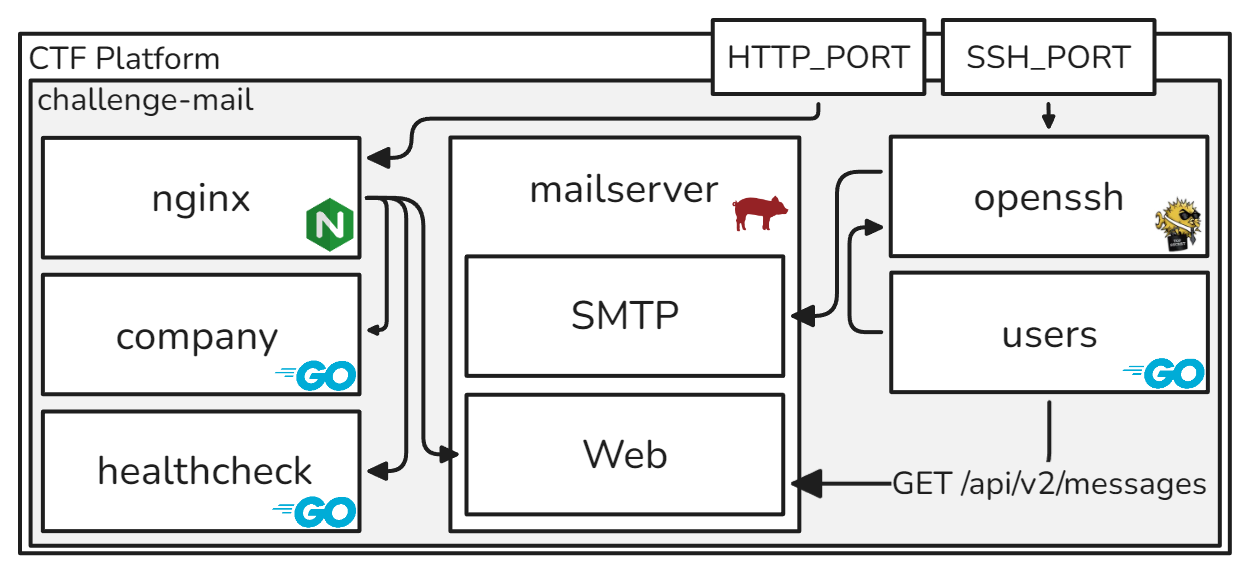
\includegraphics[width=0.9\linewidth]{img/challenge-mail--architecture.png}
    \vspace{-1\baselineskip} % Justerer afstanden mellem tekst og liste
    \caption{Mail challenge architecture}
    \label{fig:mail-architecture}
\end{figure}
\noindent
We then need to simulate the employees at Meridian Corp, who need to listen for emails in their "inboxes" and check if the emails they receive are valid. They should somehow send their login credentials to the player. At first, we wanted the player to set up a web page with a login form that this service could interact with, but because of time restrictions, it will just send a POST request. To send mails to MailHog, we need to set up a system that the player can SSH into. This service is exposed on the \texttt{SSH\_PORT} of the CTF platform. Here, the player will be able to send emails. The player can also run their HTTP server here, so the employees can send a POST request to it. We also have a \texttt{healthcheck} service, so the CTF platform can check if the challenge is running. This is its own service to split the functionality out from the company's webpage and the mail web UI. Since we have multiple websites, we use NGINX to direct incoming traffic to them, based on what subdomain the URL contains. It will redirect \texttt{company} to Meridian Corp's landing page and \texttt{mail} to MailHog's web interface. With no subdomain, it will redirect to \texttt{healthcheck}. NGINX will get exposed on port \texttt{HTTP\_PORT}.

\subsubsection{Implementation}

To implement the simulated users, the company website, and the healthcheck endpoint, we used the programming language Go\cite{github__golang}, version 1.23.9. Go has a powerful standard library, and it is designed to be simple to read and maintain, making it both great for web apps and backend services. We will describe the implementation of the \texttt{users} service here, as it is the most interesting. It checks \texttt{/api/v2/messages} from MailHog every five seconds. When it finds new messages it validates that the correct employee is the receiver, since all mails end up in the same "mailbox". It then validates the subject, and that the MIME-type of the email's content is \texttt{text/html}. To render the HTML content we have created the function, \texttt{html2image}, seen in Listing  \ref{lst:validatehtml}. It uses go-rod and Chromium to render and take screenshots. To render HTML content directly in a browser, without serving it from an endpoint, we can use data URLs\footnote{Data URLs come in the format: \texttt{data:[<media-type>][;base64],<data>}, so for rendering "Hi, Mom!" in a \texttt{<h1>} tag we can use the following URL: \texttt{data:text/html,<h1>Hi, Mom!</h1>}.}, by encoding the HTML content into one.

\begin{listing}[H]
  \begin{minted}[linenos]{go}
func html2image(html string, width, height int) (image.Image, error) {
    // Convert html to data url
    dataUrl := dataurl.EncodeBytes([]byte(html))
    // Open html using data url in browser
    path, has := launcher.LookPath()
    if !has {
        return nil, fmt.Errorf("could not find browser path")
    }
    u := launcher.New().Headless(true).Set("disable-dev-shm-usage").
        Set("disable-gpu").Bin(path).MustLaunch()
    page := rod.New().Trace(true).ControlURL(u).MustConnect().
            MustPage(dataUrl).MustWaitLoad()
    page.MustSetViewport(width, height, 1, false)
    // Capture screenshot
    screenshot, err := page.Screenshot(false, &proto.PageCaptureScreenshot{})
    if err != nil {
        return nil, err
    }
    return png.Decode(bytes.NewReader(screenshot))
}
       \end{minted}
  \vspace{-1.5\baselineskip} % Justerer afstanden mellem tekst og liste
 \caption{\texttt{users} service's Dockerfile}
\label{lst:validatehtml}
\end{listing}

We then launch Chromium in headless mode, set its viewport to the size of the handout image (Appendix \ref{apx:challenge-mail-handout}), go to the data URL, and take a screenshot of it. We use the flag \texttt{disable-dev-shm-usage} as it is a workaround for an issue where \texttt{/dev/shm} is too small in some virtual machine environments\cite{chrome_issue}. The \texttt{disable-gpu} is to make sure the GPU is disabled, as we don't need one for rendering. 

Now that we have the screenshot, we use a library called pixelmatch\cite{github__pixelmatch} to check the difference between the target image and the screenshot with a threshold of 25 percent. If it matches, then the email was valid, and we send our credentials to the link in the email. 

\subsubsection{Challenge Hardening}

To adhere to the principle of defense in depth that the CTF platform mentions\cite{ctf_platform_documentation}, we focused on challenge hardening for this challenge. Every container uses a non-root user to limit privileges. We use multi-stage builds to minimize the final images. We don't need Go when running services, only when building them. An example of this can be seen in Appendix \ref{apx:users-dockerfile}, where we build the \texttt{users} service and copy the executable from the builder stage to our final stage and run it. We also limit the resources the services can use using Docker Compose. We give 2 GB to the \texttt{users} service, as it needs to run Chromium, and spread the other 2 GB to the rest of the services.

For the NGINX service, we use a \texttt{nginxinc/nginx-unprivileged} image so NGINX runs as non-root\cite{github__nginx_unprivileged}. Normally, NGINX runs as root and can manage system-level resources; this is a problem if the service gets compromised.

\subsubsection{Testing}

To test if the challenge works as intended and get it verified on the CTF platform, we have created an automated test that replicates the steps the player will have to do to solve the challenge. This ensures that the challenge is solvable, as there will be at least one solution to it. The solution uses \texttt{golang.org/x/crypto/ssh}\cite{golang_ssh} to connect to the \texttt{openssh} service. Here, it sets up a Python HTTP server that accepts POST requests and sends the phishing email. The employee then validates the email and sends their username and password to the HTTP server. The password is the flag. This is then written to \texttt{/run/solution/flag.txt} so the CTF platform can verify it. We got this challenge verified on the CTF platform with the challenge ID: \texttt{698f6327-406b-4df7-b106-d5731dc36508}.

% https://www.youtube.com/channel/UCX6OQ3DkcsbYNE6H8uQQuVA
% mange tak!!!
% hello :) ❤
% BØH

\subsubsection{Difficulty Assessment}

We rate the challenge to be easy. The challenge feels like a good and fun introduction to phishing emails. The user gets to do the actual attack pretty fast (based on their speed), without knowing too much about mail servers. This was what we aimed for: to inform the player on how easy it is to clone emails that non-tech-savvy people might fall for.
